\chapter{Magnetic particle separation simulation}\label{ch:magneticParticleSeparationSimulation}

%\textit{To investigate particle movement and separation mechanisms in microfluidic channels, the computational simulation approach offers cost and turnaround time benefits, since it allows to explore and possibly eliminate numerous preliminary designs. In result, the manufacturing and testing of a host of competing microchannels or processes can be partially replaced with modelling. Moreover, the detail and specificity that simulation offers can help explore the exact trajectory of magnetic particle in any given magnetic field.}

\section{Introduction}
As discussed previously, magnetic particles can be manipulated using an external magnetic field, when in a surrounding liquid; this is known as magnetophoresis (see Chapter~\ref{ch:magnetophoretic_mobility}). The manipulation of magnetic beads allows for sorting or separation. 

In this chapter, the effect of an external magnetic field on the trajectory of magnetic beads will be simulated using the Lagrangian tracking scheme. Due to the assumed low particle concentration and small particle size, inter-particle forces can be neglected and one-way coupling can be assumed. A detailed description of the modelling approach can be found in Section~\ref{sec:magneticParticleTrajectorySimulation}.

% Since the magnetophoretic driving force of the specific magnet configuration was calculated, rather than the magnetic force on a single particle, the simulation retained the flexibility to simulate different magnetic particle properties. The magnetic force on a magnetic particle could simply be calculated by multiplying the magnetophoretic driving force with the particle's magnetophoretic mobility, which can either be obtained theoretically or experimentally. This modelling technique allowed the analysis of the effects of varying magnet configuration, particle characteristics and fluid channel geometry on the magnetic separation process.

% The continuous separation assumed a constant and continuous flow rate whereas the pulse mode had an unsteady pulsing flow, where its flow rate was completely switched off, leaving the particles time to move to their gathering positions, before being flushed out of the microfluidic separation device using a high flow rate. Thereby, the flushing flow rate was kept in the laminar regime, where it could be assumed that no turbulences occur and that all particles still follow their streamlines perfectly. 

\section{Continuous separation of the two novel magnet configurations}
\label{sec:continuousMagneticSeparationEfficiencyOfTheTwoNovelMagnetConfigurations}
The separation efficiency of the two presented magnet configurations (see Chapter~\ref{ch:magneticSeparationConfiguration}) is simulated and experimentally verified. Two separation strategies are introduced and investigated: \textit{continuous} mode and \textit{pulse} mode. 

The separation efficiency of both magnet configurations are evaluated by using a Monte Carlo method where $400$ individual bead trajectories are evaluated, as described in Section~\ref{sec:magneticParticleTrajectorySimulation} and Section~\ref{sec:magneticSeparationEfficiency}. Depending on the magnetic configuration the beads are introduced through the centre inlet (inlet 2 in Figure~\ref{fig:particleInletAndOutletSchematic_double}) and assumed to leave outlet 1, or through the sheath flow inlets (inlet 1 and inlet 3 in Figure~\ref{fig:particleInletAndOutletSchematic_quadrupole}) and exit through outlet 2 for the Double Magnet or Quadrupole configuration, respectively. 

\begin{figure}[htb]
	\centering
    \begin{subfigure}[b]{0.48\textwidth}
	    \centering
        \includegraphics[height=10cm]{img/chapters/chapter_7_separation_efficiency/particleInletAndOutletSchematic_double.eps}
        \caption{Double Magnet configuration}
        \label{fig:particleInletAndOutletSchematic_double}
    \end{subfigure}
    \hfill
    \begin{subfigure}[b]{0.48\textwidth}
	    \centering
        \includegraphics[height=10cm]{img/chapters/chapter_7_separation_efficiency/particleInletAndOutletSchematic_quadrupole.eps}
        \caption{Quadrupole configuration}
        \label{fig:particleInletAndOutletSchematic_quadrupole}
    \end{subfigure}
\caption[Particle inlet and outlet schematic]{Schematic showing where magnetic beads are introduced into the iBidi separation device and where they expect to exit for the two different magnet configurations. (a) In the case of the Double Magnet configuration, magnetic beads are introduced through the centre inlet (inlet 2) and are considered separated if they exit through outlet 1. (b) For the Quadrupole configuration, magnetic beads are introduced through the two sheath flows (inlet 1 and inlet 3) and are expected to exit the device through outlet 2. The green shading indicates where beads are considered separated for each configuration.}
\label{fig:particleInletAndOutletSchematic}
\end{figure}

The performance of the two magnet configurations used with the microfluidic separation device is determined by their collection efficiency $\zeta$, which can be formulated in either absolute or relative terms. The absolute separation efficiency, $\zeta_{a}$, is defined by the fraction of magnetic particles that enter the separation channel and leave the channel through the designated exit, whereas the relative separation efficiency, $\zeta_{r}$, takes the ratio of the number of particles exiting the designated channel over the total number of particles from all exits. The two separation efficiencies can be mathematically expressed as follows:
\begin{eqnarray}
    \zeta_{a} = \frac{N_{out}^{k}}{N_{in}} \\
    \zeta_{r} = \frac{N_{out}^{k}}{N_{out}}
    \label{eqn:separationEfficiency}
\end{eqnarray}

where $N_{in}$ and $N_{out}$ are the total number of particles entering and leaving the system, respectively and $N_{out}^{k}$ is the number of particles leaving the designated exit $k$. In this study, the relative separation efficiency will be simply referred to as \textit{separation efficiency} if not stated otherwise.

\subsection{Magnetic separation using the Double Magnet configuration}
The separation efficiency of the novel Double Magnet configuration presented in Chapter~\ref{ch:magneticSeparationConfiguration} is simulated as described in Section~\ref{subsec:separationEfficiencySimulation}. In the simulation, magnetic particles enter the iBidi $\mu$-Slide III 3in3 separation device through inlet 2 and are considered to be separated as soon as they have moved into the highlighted area (green highlight) in Figure~\ref{fig:particleInletAndOutletSchematic_double} and have reached the end of the fluid channel. Bead trajectories that touch the inner surface of the channel are terminated and those particles are considered to be trapped in approximately zero flow rate due to the no-slip boundary condition. 

The individual trajectories of beads moving along the separation device have been computed. Figure~\ref{fig:scatterPlotDoubleMagnetConfiguration} shows the initial and final position of the magnetic beads across the channel cross-section, after their trajectory simulation has completed or terminated. Only the top half of the fluid channel ($|y| \leq 0.2]$ mm) is simulated. The different colours show beads (i) which reach the end of the channel and are successfully separated (green), (ii) reach the end of the channel but do not get separated (blue), (iii) get successfully separated but get trapped at the top of the channel surface (orange) or (iv) do not get separated and get trapped (red).

\begin{figure}[htb!]
        \centering
        \begin{subfigure}[b]{0.45\textwidth}
                \includegraphics[width=\textwidth]{img/chapters/chapter_7_separation_efficiency/scatterPlotDoubleMagnetConfiguration_M270_30ulmin_color.eps}
                \caption{$30$ $\mu$L/min}  
        \end{subfigure}
        \hfill
        \begin{subfigure}[b]{0.45\textwidth}
                \includegraphics[width=\textwidth]{img/chapters/chapter_7_separation_efficiency/scatterPlotDoubleMagnetConfiguration_M270_50ulmin_color.eps}
                \caption{$50$ $\mu$L/min}                
        \end{subfigure}
        \hfill
        \begin{subfigure}[b]{0.45\textwidth}
                \includegraphics[width=\textwidth]{img/chapters/chapter_7_separation_efficiency/scatterPlotDoubleMagnetConfiguration_M270_150ulmin_color.eps}
                \caption{$150$ $\mu$L/min}
        \end{subfigure}
        \hfill
        \begin{subfigure}[b]{0.45\textwidth}
                \includegraphics[width=\textwidth]{img/chapters/chapter_7_separation_efficiency/scatterPlotDoubleMagnetConfiguration_M270_300ulmin_color.eps}
                \caption{$300$ $\mu$L/min}
        \end{subfigure}
        \caption[Scatter plot of starting and end position of magnetic particles for different flow rates using the Double Magnet configuration]{Scatter plot of the starting and end position of the bead trajectories for different flow rates ranging from $30$ $\mu$L/min to $300$ $\mu$L ($\bar{u}_{p}\approx 0.4-4.2$ mm/s) in (a)-(d). The open circles represent the starting position and the filled circles show their final position. The simulation is for the Double Magnet configuration while the particles have the properties of Chemicell SiMAG beads. The different colours correspond to the following: \textit{green}-beads reach the end of the channel and get successfully separated, \textit{blue}-beads reach the end of the channel but do not get separated, \textit{orange}-beads get successfully separated but get trapped at the channel surface and \textit{red}-beads do not get separated and get trapped. Higher separation efficiency is indicated by a large number of solid green beads compared to the total of solid green and blue beads.}
        \label{fig:scatterPlotDoubleMagnetConfiguration}
\end{figure}

Considering Figure~\ref{fig:scatterPlotDoubleMagnetConfiguration} it is evident that a limited number of beads are separated. Only beads entering at specific positions across the inlet (green circles) are drawn into the buffer flow without terminating at one of the internal surfaces of the channel; there is a unique area of success across the inlet cross section, which is also flow rate dependent. The reason why some beads are trapped is due to the vertical forces acting on the beads, causing them to drift upward toward the no-slip boundary condition at the channel wall. Thus, beads that touch the surface no longer move forward and are considered as trapped

Figure~\ref{fig:separationAndThroughput_beadTypes_color} presents the simulated separation efficiency and bead throughput of the Double Magnet configuration for the different magnetic bead types at different continuous flow rates. The susceptibilities are set to the values found in the bead magnetization study (see Section~\ref{sec:magnetizationOfSuperparamagneticParticles}) and also adjusted according to the local magnetic field strength during the simulation.

\begin{figure}[htb]
\centering
    \begin{subfigure}[b]{0.48\textwidth}
         \includegraphics[width=\textwidth]{img/chapters/chapter_7_separation_efficiency/relativeSeparationEfficiencyDoubleMagnetConfiguration_beadTypes-line_color.eps}
        \caption{}
        \label{fig:relativeSeparationEfficiencyDoubleMagnetConfiguration_beadTypes_color}
    \end{subfigure}
    \hfill
    \begin{subfigure}[b]{0.48\textwidth}
         \includegraphics[width=\textwidth]{img/chapters/chapter_7_separation_efficiency/throughputDoubleMagnetConfiguration_beadTypes-line_color.eps}
        \caption{}
        \label{fig:throughputDoubleMagnetConfiguration_beadTypes_color}
    \end{subfigure}
\caption[Relative magnetic separation efficiency and throughput of the analysed magnetic bead types for different flow rates using the Double Magnet configuration]{(a) Continuous separation efficiency and (b) throughput of the Double Magnet configuration for different bead types and flow rates. The flow rates range between $10$ $\mu$L/min ($\bar{u}_{p}\approx0.14$ mm/s) to $375$ $\mu$L/min ($\bar{u}_{p}\approx5.2$ mm/s). The bead properties are set to the physical properties found in Chapter~\ref{ch:magnetophoretic_mobility}.}
\label{fig:separationAndThroughput_beadTypes_color}
\end{figure}

It can be noted in Figure~\ref{fig:separationAndThroughput_beadTypes_color}, that the separation efficiency and the particle throughput are inversely proportional. Also, using beads of higher magnetophoretic mobility improves the separation efficiency, with reduced throughput; i.e. there is a trade-off between the separation efficiency and throughput. For example, to have a separation efficiency of approximately $80\%$, which is comparable to separation efficiencies found in the literature, about $30\%$ of the introduced beads can be collected at the designated outlet (see Figure~\ref{fig:separationAndThroughput_beadTypes_color}).

The results obtained by simulation have been experimentally verified for various flow rates, as described in Section~\ref{subsec:separationEfficiencyExperiment}. In these experiments SiMAG-Silanol beads (Chemicell) were used because they have a high magnetophoretic mobility (see Chapter~\ref{ch:magnetophoretic_mobility}) and sediment slower than Dynabeads M270. As described in Chapter~\ref{ch:experiments}, a bead concentration of $10^{6}$ beads/mL ($\upsilon_{p}\approx10^-7$) was used for the suspension, which is considered as a low concentration because $\upsilon_{p}<10^-6$ (see Chapter~\ref{subsec:particleLadenFlowInMicrofluidicSystems}).

Observations recorded with the CCD camera show a visible separation in the experiment and that the magnetic beads are continuously deflected by the magnet from the central sample flow into the buffer flow, as shown in Figure~\ref{fig:continuousMagneticSeparationExperimentDoubleMagnet}. This demonstrates that separation of magnetic beads is achieved. 

\begin{figure}[htb]
   \centering
   \includegraphics[width=0.9\textwidth]{img/chapters/chapter_7_separation_efficiency/magneticBeadStreamlinesIbidiDoubleMagnet_ink_4images.pdf}
   \caption[Magnetic separation experiment of the Double Magnet configuration in continuous flow]{Gathering and streamlines of superimposed images of magnetic beads (Chemicell SiMAG) during the continuous magnetic separation experiment with the Double Magnet configuration. Magnetic beads are introduced through inlet 2 and expected to exit the device through outlet 1. Images (a)-(d) show the streamlines of the magnetic beads at different positions along the iBidi fluid channel when a flow rate of $150$ $\mu$L/min is applied. The flow direction at the inlets and outlets is indicated by the bold arrows in (a) and (d). }
   \label{fig:continuousMagneticSeparationExperimentDoubleMagnet}
\end{figure}

The separation efficiency of the separation configuration using the Double Magnet was determined by analysing the collected outlet samples using flow cytometry. At flow rates $\leq30$ $\mu$L/min ($\bar{u}_{p}\approx0.4$ mm/s), no beads were detected at any of the three outlets. Therefore, a higher flow rate ($>30$ $\mu$L/min) is needed for a viable throughput. Measuring the samples at the three outlet channels at total flow rates $>150$ $\mu$L/min indicates that more than $55\%$ of magnetic beads had not been sufficiently deflected from the main sample flow and thus, not separated. These beads travelled through the device along their streamlines and exited through outlet 2, as depicted in Figure~\ref{fig:relativeSeparationEfficiencyContineousExperimentDoubleConfiguration}. This shows that an interaction time with the magnets of approximately $\approx10$ seconds has not been enough to draw the particles from the sample into the buffer flow. A more detailed view of the continuous separation in Figure~\ref{fig:relativeSeparationEfficiencyContineousExperimentDoubleConfiguration} can be found in Appendix~\ref{sec:magneticBeadSeparationAppendix}.

\begin{figure}[htb]
   \centering
   \includegraphics[width=0.7\textwidth]{img/chapters/chapter_7_separation_efficiency/relativeSeparationEfficiencyExperimentHistogram_color.eps}
   \caption[Experimental magnetic bead separation efficiency of the Double Magnet configuration in continuous flow]{Experimental results of continuous separation efficiencies with the Double Magnet configuration for different flow rates. The flow rates stated here are the sum of all inlet flow rates while keeping their inlet flow rate ratios at $1:1:1$ across the different inlets. The experiment has been repeated $3$ times for all shown flow rates.}
   \label{fig:relativeSeparationEfficiencyContineousExperimentDoubleConfiguration}
\end{figure}

As expected from the numerical simulations, the separation efficiency of the Double Magnet configuration is found to be negatively correlated with the total flow rate (see Figure~\ref{fig:relativeSeparationEfficiencyContineousExperimentDoubleConfiguration}). The results of the experimental separation efficiency for the Double Magnet configuration, however, are $10\%-15\%$ higher compared to the simulation at corresponding flow rates. The better performance is most likely due to the fact that in the experiment, beads have a tendency to agglomerate and are then deflected more quickly than individual beads; this is an effect not currently modelled. The samples collected for the flow cytometer were ultrasonicated prior to the measurement to break up bead agglomerates, and therefore would have been counted as individual beads in the sample analysis. For flow rates $>375$ $\mu$L/min ($\bar{u}_{p}\approx5.2$ mm/s), the separation efficiency of the model and the experiments are comparable, because the fluid dynamics becomes the dominant factor whereas the effect of agglomerates are less significant.

The clearly visible separation, apparent in the photograph of Figure~\ref{fig:continuousMagneticSeparationExperimentDoubleMagnet}, suggests that an even higher separation efficiency should be obtained compared with that determined from the bead count, i.e. the beads appear to be strongly gathered due to the dark band in the image, but the flow cytometer measurements did not support the anticipated separation efficiency. Further examination using higher magnification revealed beads and agglomerations \textit{stuck} at the top or the bottom of the channel due to the vertical magnetic forces, leading to a bold band of stationary beads. It is assumed that the distribution of the beads across the entire area of cross-section of the inlet channel and possible misalignment of the magnets contributed to the lower than expected performance.

Based on the observations in the experiments the effect of bead agglomerates as well as magnet displacement errors is simulated in the following sections. Further, the influence of a cell cargo attached to a magnetic bead is investigated.

\subsubsection{Effects of magnetic bead agglomerates}
\label{subsec:particleTrajectoriesOfAgglomerates}
As soon as superparamagnetic beads are exposed to a magnetic field, they become magnetized and start attracting other magnetic particles in their vicinity. This causes beads to form agglomerates as can be observed in the magnetophoretic study for magnetic bead agglomerates (see Chapter~\ref{ch:magnetophoretic_mobility}). Even when starting from a fully suspended sample at low concentration ($\approx10^{6}$ beads/mL), bead agglomerates can quickly form and bead-bead interactions can occur if beads happen to be close enough. Therefore, in order to understand the behaviour of more complex suspensions the trajectories of bead aggregates also needs to be studied. 
 
The bead agglomerate model presented in Section~\ref{sec:magnetophoreticMobilityOfSuperparamagneticAgglomerates} shows that the drag force on a chain of beads does not increase linearly with the number of beads, but its magnetic force does. This model is implemented in the simulation. Bead chains of up to $5$ beads are studied here. Figure~\ref{fig:relativeSeparationEfficiencyAndParticleThroughputDoubleMagnetConfigurationAgglomerations} shows the separation efficiency and throughput for different agglomerate sizes and flow rates.

\begin{figure}[htb]
        \centering
        \begin{subfigure}[b]{0.48\textwidth}
                \includegraphics[width=\textwidth]{img/chapters/chapter_7_separation_efficiency/relativeSeparationEfficiencyDoubleMagnetConfiguration_agglomerations-line_color.eps}
                \caption{}  
                \label{fig:relativeSeparationEfficiencyDoubleMagnetConfigurationAgglomerations}
        \end{subfigure}
        \hfill
        \begin{subfigure}[b]{0.48\textwidth}
                \includegraphics[width=\textwidth]{img/chapters/chapter_7_separation_efficiency/throughputDoubleMagnetConfiguration_agglomerations-line_color.eps}
                \caption{}       
                \label{fig:particleThroughputDoubleMagnetConfigurationAgglomerations}         
        \end{subfigure}
        \caption[Relative magnetic separation efficiency and throughput of magnetic bead agglomerates for different flow rates using the Double Magnet configuration]{(a) Magnetic separation efficiency and (b) throughput for different bead agglomerates using the Double Magnet configuration. The flow rates range between $30-375$ $\mu$L/min ($\bar{u}_{p}=0.4-5.2$ mm/s) in the main channel. Bead agglomerates which have crossed the $x=-0.5$ mm line without colliding with an inner surface are considered to be separated. The bead properties for a single magnetic bead are set equal to the properties of a $1.0$ $\mu$m sized SiMAG-Silanol (Chemicell) particle.}
        \label{fig:relativeSeparationEfficiencyAndParticleThroughputDoubleMagnetConfigurationAgglomerations}
\end{figure}

Larger clusters experience a higher magnetophoretic drift velocity (see Section~\ref{subsec:magneticallyInducedVelocityOnSuperparamagneticParticles}), which explains the increasing relative separation efficiency in Figure~\ref{fig:relativeSeparationEfficiencyDoubleMagnetConfigurationAgglomerations}. It is noted, however, that the increased magnetically induced velocity also causes larger clusters to get stuck at the inner surface of the fluid channel which leads to a lower overall particle throughput (see Figure~\ref{fig:particleThroughputDoubleMagnetConfigurationAgglomerations}).

\subsubsection{Effects of magnet displacement error relative to the microfluidic separation device}
\label{subsec:effectsOfMagnetMisalignment}
The specific flux density patterns seen in Chapter~\ref{ch:magneticSeparationConfiguration} are only valid as long as the microfluidic separation device (see Section~\ref{subsec:microfluidicSeparationDevice}) is correctly positioned, i.e. placed along the central plane ($y=0$) between the two magnets. If the microfluidic separation device is placed either side of this central position such that $y \geq 0.7$ mm, the gathering points vanish. Therefore, care needs to be taken when the device is assembled requiring sub-millimetre accuracy. Figure~\ref{fig:doubleMagnetConfigurationMisalignment} shows a schematic of the critical vertical displacement used in this study of misalignment error. Misalignment of the two magnets in the horizontal $x-z$ plane, such that the two magnets are offset relative to each other, is less likely because the magnetic attraction force pulls the two magnets automatically into alignment with one exactly above the other. Thus, a horizontal magnet misalignment will not be considered here.

\begin{figure}[htb]
\centering
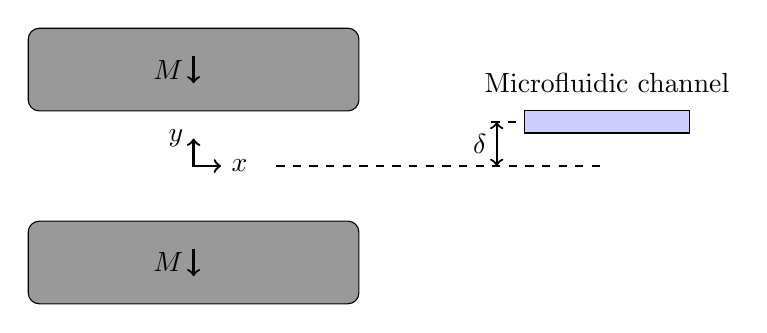
\begin{tikzpicture}[scale=0.7]
    \filldraw[rounded corners, fill=black!40!white, draw=black] (-9,1) rectangle (-3,2.5);
    \filldraw[rounded corners, fill=black!40!white, draw=black] (-9,-1) rectangle (-3,-2.5);    
    \filldraw[fill=blue!20!white, draw=black] (0,0.6) rectangle (3,1.0);    
    \node[thick] at (1.5,1.5) {Microfluidic channel };

    \draw[line width=0.3mm,<->] (-6,0.5) node[anchor=east] {$y$} -- (-6,0) -- (-5.5,0)node[anchor=west] {$x$};

    \draw[thick,dashed,-] (-4.5,0) -- (1.5,0);
    \draw[thick,dashed,-] (-0.6,0.8) -- (0,0.8);
    \draw[thick,<->] (-0.5,0) -- node[thick,anchor=east]{$\delta$} (-0.5,0.8);
    \draw[thick,->] (-6,2) -- node[thick,anchor=east]{$M$} (-6,1.5);
    \draw[thick,->] (-6,-1.5) -- node[thick,anchor=east]{$M$} (-6,-2);
\end{tikzpicture}
\caption[Schematic of vertical misalignment of the microfluidic separation device]{Schematic of vertical misalignment of the microfluidic separation device from its central plane ($y=0$) position. The parameter $\delta$ is the distance the microfluidic channel is misplaced out of the centre.}
\label{fig:doubleMagnetConfigurationMisalignment}%
\end{figure}

Performance with displacement errors of the channel in the $y$ direction at values of $\delta=100$ $\mu$m, $\delta=300$ $\mu$m and $\delta=500$ $\mu$m has been simulated; offset errors greater than $0.5$ mm were regarded as unlikely. The $\mathbf{B}$ field inside the fluid channel is no longer symmetrical about the $x$ axis due to the relative displacement of the channel compared to the magnets. Bead trajectories were simulated across the entire cross-section of the centre inlet channel (channel 2), with twice as many beads as in the previous simulations. Figure~\ref{fig:relativeSeparationEfficiencyAndParticleThroughputDoubleMagnetConfigurationMagnetOffset} shows the separation efficiency and the particle throughput for different flow rates and different channel offsets.

\begin{figure}[htb]
        \centering
        \begin{subfigure}[b]{0.48\textwidth}
                \includegraphics[width=\textwidth]{img/chapters/chapter_7_separation_efficiency/relativeSeparationEfficiencyDoubleMagnetConfiguration_missalignment-line_color.eps}
                \caption{}  
        \end{subfigure}
        \hfill
        \begin{subfigure}[b]{0.48\textwidth}
                \includegraphics[width=\textwidth]{img/chapters/chapter_7_separation_efficiency/throughputDoubleMagnetConfiguration_missalignment-line_color.eps}
                \caption{}                
        \end{subfigure}
        \caption[Relative magnetic bead separation efficiency and throughput when the microfluidic channel has a displacement compared to the two magnets of the Double Magnet configuration]{(a) Magnetic separation efficiency and (b) bead throughput for flow rates ranging between $30-375$ $\mu$L/min ($\bar{u}_{p}=0.4-5.2$ mm/s) in the main channel. The plot shows the results for a vertical displacement of the magnets of $\delta=0$ $\mu$m, $\delta=100$ $\mu$m, $\delta=300$ $\mu$m and $\delta=500$ $\mu$m.}
        \label{fig:relativeSeparationEfficiencyAndParticleThroughputDoubleMagnetConfigurationMagnetOffset}
\end{figure}

% old version
%This phenomena is caused by the fact that at high flow rates particles have less time to interact with the magnets, which requires a higher magnetic field to move the particles in a short period of time. A larger vertical offset, generates a larger magnetic field, because one of the two magnets will be closer and thus, has a larger attraction capability. This makes more particles to cross the critical line of $x=-0.5$ mm even when there is not much interaction time. 

The results in Figure~\ref{fig:relativeSeparationEfficiencyAndParticleThroughputDoubleMagnetConfigurationMagnetOffset} suggest that a small positive misalignment ($|\delta| > 0$) is advantageous for the magnetic separation process at low flow rates ($\dot{Q} \leq 100$ $\mu$L/min), while at higher flow rates ($\dot{Q} > 100$ $\mu$L/min) the effect of the misalignment becomes almost insignificant. This behaviour is caused by the fact that at higher flow rates beads have less time to interact with the magnets.

It is interesting to see that at small flow rates the relative separation efficiency is not a monotonic decreasing function with respect to the parameter $\delta$. Due to the complex force pattern, different offset values of $\delta$ result in different relative separation efficiency for different flow rates. The separation efficiency is dependent on what percentage of the cross-section of the fluid channel lies above or below the $y=0$ symmetry plane. The more the fluid channel is displaced from its symmetry position (upwards or downwards), the larger the force on the beads in the vertical direction. There is a trade-off between the number of beads separated and the number of trapped beads. A larger offset does not necessarily impact the separation efficiency, but has a strong influence on throughput.

Since the uncertainty of the particle trajectories increases with a larger displacement error, the fluid channel should be carefully positioned at $y=0$.

\subsubsection{Effects of a cell cargo attached to a magnetic bead}\label{subsec:effectsOfMagneticBeadCargo}
For magnetic cell separation, a cell will be attached to the magnetic beads as a cargo. Such biological cargo is normally nonmagnetic, or only weakly para- or diamagnetic, compared to the superparamagnetic bead~\cite{Takayasu2000,Yang1999,Zborowski2003red}. 

For a cell bound to a magnetic bead, the model given in Equation~\ref{eqn:parallel} and Equation~\ref{eqn:perpendicular} predicts a smaller magnetophoretic drift velocity, and thus mobility, for the bead complex as a whole compared to a single magnetic bead. Wise \etal{} found that the magnetophoretic mobility of $1.05-2.8$ $\mu$m sized magnetic beads with a single $1.0$ $\mu$m sized nonmagnetic spherical particle attached is reduced by $15-25\%$~\cite{WisePhD2015}. The mobility of the bead complex is further reduced with increasing number of attachments of nonmagnetic particles and their diameter. Additionally, Wise \etal{} compared the magnetophoretic mobility of Dynabeads MyOne microspheres, when attached to single living and dead \textit{E. coli} bacteria. Such cell-bead complexes were observed to travel at a velocity approximately $49\%$ (living) and $75\%$ (dead) of that of a single bead with no cell cargo. In all cases observed, the nonmagnetic attachment aligned behind the magnetic bead in the direction of travel to reduce drag~\cite{WisePhD2015}.

Figure~\ref{fig:relativeSeparationEfficiencyAndParticleThroughputDoubleMagnetConfigurationCellCargo} shows the relative separation efficiency and throughput for Dynabeads MyOne microspheres when they have a living or dead cell bound to them. For comparison, the data is also presented for an individual Dynabeads MyOne microsphere with no cell cargo attached.

\begin{figure}[htb]
        \centering
        \begin{subfigure}[b]{0.48\textwidth}
                \includegraphics[width=\textwidth]{img/chapters/chapter_7_separation_efficiency/relativeSeparationEfficiencyDoubleMagnetConfiguration_cellCargo-line_color.eps}
                \caption{}  
                \label{fig:relativeSeparationEfficiencyDoubleMagnetConfigurationCellCargo}
        \end{subfigure}
        \hfill
        \begin{subfigure}[b]{0.48\textwidth}
                \includegraphics[width=\textwidth]{img/chapters/chapter_7_separation_efficiency/throughputDoubleMagnetConfiguration_cellCargo-line_color.eps}
                \caption{}       
                \label{fig:particleThroughputDoubleMagnetConfigurationCellCargo}         
        \end{subfigure}
        \caption[Relative magnetic separation efficiency and throughput when a viable or non-viable cell cargo is attached to a magnetic bead for different flow rates using the Double Magnet configuration]{(a) Magnetic separation efficiency and (b) throughput for different total flow rates, ranging between $30-375$ $\mu$L/min ($\bar{u}_{p}=0.4-5.2$ mm/s) in the main channel for beads with a viable or non-viable \textit{E. coli} bacteria attached to a magnetic bead. The simulation is done for the Double Magnet configuration with the bead and mobility properties set to the experimentally found properties for Dynabeads MyOne in Chapter~\ref{ch:magnetophoretic_mobility} and by Wise \etal{}~\cite{WisePhD2015}.}
        \label{fig:relativeSeparationEfficiencyAndParticleThroughputDoubleMagnetConfigurationCellCargo}
\end{figure}

\subsection{Magnetic separation using the Quadrupole configuration}\label{subsec:continuousMagneticSeparationUsingTheQuadrupoleConfiguration}
The Quadrupole configuration has potential for improved separation efficiencies due to its higher magnetophoretic force compared to the Double Magnet configuration (see Section~\ref{subsec:quadrupoleMagnetConfiguration}). However, there are higher vertical ($y$ direction) forces, causing more beads to become trapped in the system. In order to investigate the vertical forces, three different magnet geometries for the Quadrupole configuration are modelled; simple bar magnet, tapered magnet and parabolic magnet. The three magnet geometries  are shown in Figure~\ref{fig:relativeSeparationEfficiencyAndParticleThroughputQuadrupoleMagnetConfigurationMagnetGeometries}(a). Figure~\ref{fig:relativeSeparationEfficiencyAndParticleThroughputQuadrupoleMagnetConfigurationMagnetGeometries}(b)-\ref{fig:relativeSeparationEfficiencyAndParticleThroughputQuadrupoleMagnetConfigurationMagnetGeometries}(c) show the simulated separation efficiencies and the corresponding particle throughput of the various magnet shapes derived from the models. The trajectories are simulated as outlined in Section~\ref{subsec:separationEfficiencySimulation} with the particles introduced in inlet 1, and separated from the sample flow into channel 2, as shown in Figure~\ref{fig:particleInletAndOutletSchematic_quadrupole}.

\begin{figure}[htb!]
    \centering
    \includegraphics[width=\textwidth]{img/chapters/chapter_7_separation_efficiency/relativeSeparationEfficiencyAndThroughputQuadrupoleMagnetConfiguration_geometry_color.eps}
        \caption[Relative magnetic separation efficiency and throughput for different flow rates using different magnet geometries for the Quadrupole configuration]{(a) Shows the different magnet geometries used to assemble the Quadrupole configuration. Only one side of the Quadrupole configuration is shown for simplicity. Simulation of (b) the relative magnetic separation efficiency and (c) throughput in continuous flow for Quadrupole configurations with three different magnet geometries. The flow rates range between $10$ $\mu$L/min ($\bar{u}_{p}\approx0.14$ mm/s) to $375$ $\mu$L/min ($\bar{u}_{p}\approx5.2$ mm/s). The bead properties are set to the physical properties of Chemicell SiMAG beads, found in Chapter~\ref{ch:magnetophoretic_mobility}.}
        \label{fig:relativeSeparationEfficiencyAndParticleThroughputQuadrupoleMagnetConfigurationMagnetGeometries}
\end{figure}

Each magnet geometry in Figure~\ref{fig:relativeSeparationEfficiencyAndParticleThroughputQuadrupoleMagnetConfigurationMagnetGeometries}(a) generates a different magnetic flux field and magnitude. The parabolic magnet generates a smaller horizontal magnetic driving force than the tapered or bar magnet and therefore has a lower separation efficiency across most flow rates, however, the parabolic shape reduces vertical forces on the magnetic particle, which improves particle throughput, as shown in Figure~\ref{fig:relativeSeparationEfficiencyAndParticleThroughputQuadrupoleMagnetConfigurationMagnetGeometries}(b)-\ref{fig:relativeSeparationEfficiencyAndParticleThroughputQuadrupoleMagnetConfigurationMagnetGeometries}(c). For example, at a flow rate of $100$ $\mu$L/min ($\bar{u}_{p}\approx1.4$ mm/s), a continuous separation efficiency of $100\%$ and a $17\%$ particle throughput is predicted in the simulation with the parabolic magnet geometry, whereas no beads can be recovered when simulating the tapered or bar magnet geometry under the same flow conditions. For comparison, the tapered and bar magnet geometry achieve a continuous relative separation efficiency of $100\%$ at a flow rate of $225$ $\mu$L/min ($\bar{u}_{p}\approx3.1$ mm/s), but the particle throughput is reduced to $14.5\%$ and $13.7\%$, respectively. 

With increasing flow rate, the separation efficiency of all three magnet geometries reduces. The reduction in separation efficiency is most significant for the parabolic magnet geometry. This, on the other hand, increases the throughput of beads which can be collected and recycled through another separation cycle. 

Compared to the simple Double Magnet configuration (see Figure~\ref{fig:separationAndThroughput_beadTypes_color}), all three Quadrupole simulations can achieve a maximum separation efficiency of $100\%$ with higher throughput at higher flow rates, which essentially reduces separation processing time. This evaluation is for separation of Chemicell SiMAG beads. The magnetic separation efficiency and throughput are, as with the Double Magnet configuration, negatively correlated. Therefore, the simulations predict again a trade-off between the continuous separation efficiency and bead recovery for each Quadrupole configuration. 

The continuous separation of the Quadrupole configuration with bar magnets is also experimentally tested, as described in Section~\ref{subsec:separationEfficiencyExperiment}. Figure~\ref{fig:continuousMagneticSeparationExperimentQuadrupole} shows the streamlines of the magnetic beads in continuous flow. A maximum separation efficiency of $55\%$ has been achieved when run continuously at a flow rate of $39$ $\mu$L/min ($\bar{u}_{p}\approx0.5$ mm/s). 

\begin{figure}[htb]
   \centering
   \includegraphics[width=0.9\textwidth]{img/chapters/chapter_7_separation_efficiency/magneticBeadStreamlinesIbidiQuadrupole_ink_4images.pdf}
   \caption[Magnetic separation experiment of the Quadrupole configuration in continuous flow]{Gathering and streamlines of superimposed images of magnetic beads (Chemicell SiMAG) during the continuous magnetic separation experiment with the Quadrupole configuration. Images (a)-(d) show the streamlines of the magnetic beads at different positions along the iBidi fluid channel. The position of the various stages of the separation process is indicated by the black rectangles. Magnetic beads are introduced through inlet 1 only, for simplicity, and are expected to exit the device through outlet 2. The flow direction at the inlets and outlets is indicated by the bold arrows in (a) and (d).}
   \label{fig:continuousMagneticSeparationExperimentQuadrupole}
\end{figure}

%The experimentally determined separation efficiency of $55\%$ shows that separation under continuous flow does work but might need to be run in sequence to allow enough time for all magnetic beads to migrate into the central outlet and most beads have still been detected in the outlets (outlet 1 or outlet 3) along the streamlines of their introductory inlets (inlet 1 or inlet 3). 

As seen from the simulations and experiments, the Quadrupole configuration has the ability to continuously isolate magnetic beads and has proved more successful compared to both the experiments and simulations using the Double Magnet configuration. The experimentally found separation efficiency of the Quadrupole configuration for the tested flow rate is approximately half of what has been predicted by the simulations. The visually observed separation in the experiments lead to the conclusion that beads are getting separated, but cannot be collected. It is assumed that beads are getting trapped in the channel, because they move towards areas of low fluid velocity at the surface of the channel. Therefore, the impact of beads approaching the inner surface of the fluid channel needs further attention, which is the topic in the next section.

\section{Wall effects on the motion of a single particle}
\label{sec:wallEffectsOnTheMotionOfASingleParticle}
In the evaluations so far, the throughput is affected by beads becoming stuck at the fluid channel's inner surface, due to the undesirable vertical magnetophoretic forces. Thus, the motion of a rigid sphere in the vicinity of an internal wall might be relevant to this study. Therefore, the effect on the bead's motion when approaching a single plane wall is considered here. 

\begin{figure}[htb]
\centering
\begin{subfigure}[b]{0.48\textwidth}
\centering
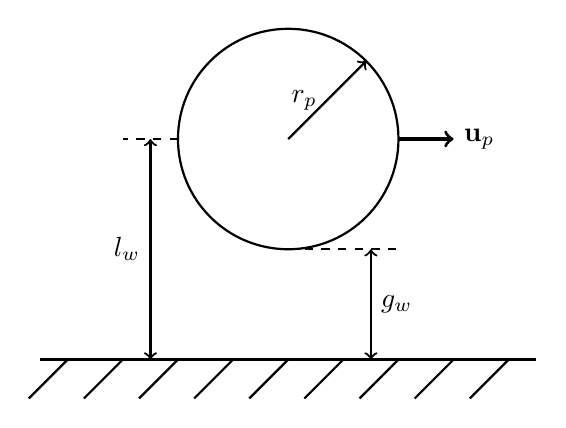
\begin{tikzpicture}[scale=0.7]
\draw[thick] (-4.5,0) -- (4.5,0);
\foreach \x in {-4,...,4} 
  \draw[thick] (\x-0.7071,-0.7071) -- (\x,0);
  
\draw[thick] (0,4) circle (2);
\draw[thick,->] (0,4) -- node[thick,anchor=east]{$r_{p}$} (1.4142,4+1.4142);
\draw[thick,dashed] (-2,4) -- (-3,4);
\draw[thick,<->] (-2.5,0) -- node[thick,anchor=east]{$l_{w}$} (-2.5,4);
\draw[thick,dashed] (0,2) -- (2,2);
\draw[thick,<->] (1.5,0) -- node[thick,anchor=west]{$g_{w}$} (1.5,2);

\draw[very thick,->] (2,4) -- (3,4) node[thick,anchor=west]{$\mathbf{u}_{p}$};
\end{tikzpicture}
\caption{} 
\end{subfigure}
\hfill
\begin{subfigure}[b]{0.48\textwidth}
\centering
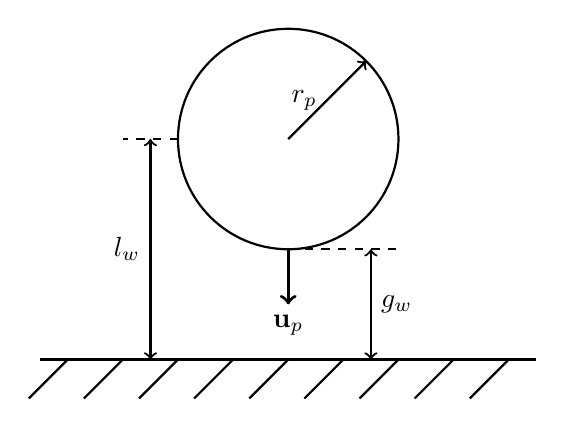
\begin{tikzpicture}[scale=0.7]
\draw[thick] (-4.5,0) -- (4.5,0);
\foreach \x in {-4,...,4} 
  \draw[thick] (\x-0.7071,-0.7071) -- (\x,0);
  
\draw[thick] (0,4) circle (2);
\draw[thick,->] (0,4) -- node[thick,anchor=east]{$r_{p}$} (1.4142,4+1.4142);
\draw[thick,dashed] (-2,4) -- (-3,4);
\draw[thick,<->] (-2.5,0) -- node[thick,anchor=east]{$l_{w}$} (-2.5,4);
\draw[thick,dashed] (0,2) -- (2,2);
\draw[thick,<->] (1.5,0) -- node[thick,anchor=west]{$g_{w}$} (1.5,2);

\draw[very thick,->] (0,2) -- (0,1) node[thick,anchor=north]{$\mathbf{u}_{p}$};
\end{tikzpicture}
\caption{} 
\end{subfigure}
\caption[Schematic of spherical beads moving in proximity to a planar wall]{Spherical beads moving in proximity to a single plane wall experience different hydrodynamic forces when they move (a) along or (b) towards the wall.}
\label{fig:particleMotionCloseToWall}
\end{figure}

Beads can move either along or towards the solid wall as shown in Figure~\ref{fig:particleMotionCloseToWall}. In either case, the hydrodynamic forces on the object change when the object moves in close proximity to the wall. In order to account for this effect, the magnetophoretic drift velocity should be adjusted. This is done by adding a correction factor, $\beta$, to the Stokes drag~\cite{Faxen1922,Brenner1961}:
\begin{equation}
    \mathbf{F}_{D} = 6\pi\eta_{f} r_{p} \mathbf{u} \beta
    \label{eqn:wallEffectCorrectedDragForce}
\end{equation}

Faxen worked out the influence of a single plane wall for spherical particles moving parallel to the wall and Brenner developed the model of a sphere moving towards a solid wall. The two Stokes' law correction factors for a spherical particle moving parallel ($\beta_{\parallel}$) or perpendicular ($\beta_{\perp}$) to a plane wall can be given by~\cite{Faxen1922,Brenner1961}:
\begin{eqnarray}
    \beta_{\parallel} &=& \frac{1}{1-\Big(\frac{9}{16}\Big)\left(\frac{r_{p}}{l_{w}}\right)+\Big(\frac{1}{8}\Big)\left(\frac{r_{p}}{l_{w}}\right)^{3}-\Big(\frac{45}{256}\Big)\left(\frac{r_{p}}{l_{w}}\right)^{4}-\Big(\frac{1}{6}\Big)\left(\frac{r_{p}}{l_{w}}\right)^{5}} \\
    \beta_{\perp} &=& \frac{4}{3} \sinh(\varphi) \sum_{n=1}^{\infty} \frac{n(n+1)}{(2n-1)(2n+3)} \times \\
     && \left[ \frac{2\sinh(2n+1)\varphi + (2n+1\sinh(2\varphi))}{4\sinh^{2}(n+0.5)\varphi-(2n+1)^{2}\sinh^{2}(\varphi)} -1\right] \nonumber
    \label{eqn:wallEffectCorrectionFactors}
\end{eqnarray}
where the particle radius is denoted by $r_{p}$ and the distance of its midpoint from the plane by $l_{w}$, as depicted in Figure~\ref{fig:particleMotionCloseToWall}. The parameter $\varphi$ is given by the following relationship:
\begin{equation}
     \varphi = \cosh^{-1}(l_{w}/r_{p})
     \label{eqn:radiusToDistanceToPlane}
\end{equation}

Figure~\ref{fig:wallCorrectionFactors} shows the two correction factors, $\beta_{\parallel}$ and $\beta_{\perp}$, for a spherical particle moving at different distances away from a single wall. It can be seen that the correction factor approaches a constant value ($\beta_{\parallel}\approx 3$) when the particle is moving in close proximity to a wall (Figure~\ref{fig:wallCorrectionFactorsParallel}), whereas in the perpendicular case, the drag force correction factor increases infinitely (Figure~\ref{fig:wallCorrectionFactorsPerpendicular}). This means that a rigid spherical particle in a viscous fluid can never make contact with a solid surface in a finite time. In practice, this is due to the lubrication force when the distance approaches zero~\cite{Brenner1961,Cox1967,Davis1986}.% A film thickness of $1$ nm between the particle and the wall can be assumed~\cite{Lin2013}. % check this statement

\begin{figure}[htb]
        \centering
        \begin{subfigure}[b]{0.48\textwidth}
                \includegraphics[width=\textwidth]{img/chapters/chapter_7_separation_efficiency/wallDragForcCorrectionFactorParallel2.eps}
                \caption{}
                \label{fig:wallCorrectionFactorsParallel}
        \end{subfigure}     
        \hfill                   
        \begin{subfigure}[b]{0.48\textwidth}
                \includegraphics[width=\textwidth]{img/chapters/chapter_7_separation_efficiency/wallDragForcCorrectionFactorPerpendicular2.eps}
                \caption{}
                \label{fig:wallCorrectionFactorsPerpendicular}
        \end{subfigure}         
        \caption[Wall correction factor for rigid sphere in proximity to a planar wall]{Wall correction factors for different distances from a plane surface for when a rigid sphere is moving (a) parallel or (b) perpendicular to the surface.}
        \label{fig:wallCorrectionFactors}
\end{figure}

Particles that are travelling close to an internal surface of the microfluidic channel slow down in velocity because of the no-slip condition of the parabolic velocity profile of the fluid. Due to their finite size, as shown in Figure~\ref{fig:particleStuckAtPlanarSurfaceVelocity}, the mean velocity of a particle which is at the channel's surface can be approximated by integrating Equation~\ref{eqn:velocityProfileRectangularDuct} along the diameter of the particle. The thin layer of liquid between the particle and wall that might be present in practice is assumed to be negligible compared to the particle diameter.

It is found that the bead's mean velocity, when moving along the wall, is more than $100$ times smaller than the mean fluid velocity in the channel. Consequently, it takes at least $100$ times longer for these beads to exit the separation device. This confirms the observation found through experiment, i.e. beads can be assumed as trapped on the time scale of continuous flow operation.

\begin{figure}[htb]
\centering
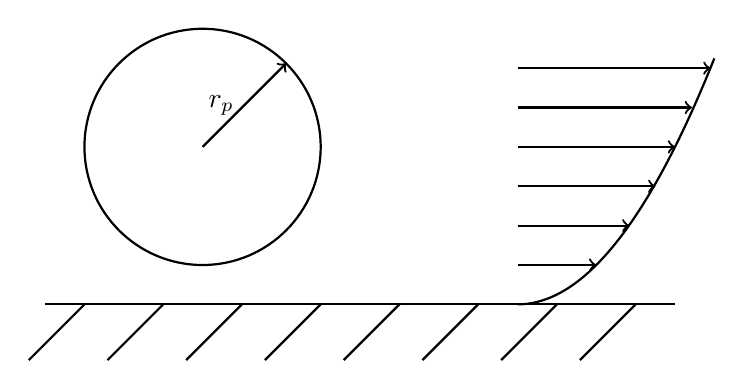
\begin{tikzpicture}[scale=1.0]
\draw[thick] (-6,0) -- (2,0);
\foreach \x in {-5.5,...,1.5} 
  \draw[thick] (\x-0.7071,-0.7071) -- (\x,0);
  
\draw[thick] (-4,2) circle (1.5);
\draw[thick,->] (-4,2) -- node[thick,anchor=east]{$r_{p}$} (-4+0.7071*1.5,2+0.7071*1.5);

\draw[thick,scale=1,domain=0:2.5,smooth,variable=\x] plot ({\x},{0.5*\x*\x});
\draw[thick,->] (0,0.5) -- (1.0,0.5);
\draw[thick,->] (0,1.0) -- (1.42,1.0);
\draw[thick,->] (0,1.5) -- (1.75,1.5);
\draw[thick,->] (0,2.0) -- (2.0,2.0);
\draw[thick,->] (0,2.5) -- (2.215,2.5);
\draw[thick,->] (0,3.0) -- (2.45,3.0);
\end{tikzpicture}
\caption[Schematic of spherical particle in a flow field in proximity to a planar wall]{A spherical particle in a flow field in close proximity to a planar will experience a higher drag force due to its finite size.}
\label{fig:particleStuckAtPlanarSurfaceVelocity}
\end{figure}

However, it can be experimentally shown that beads can be flushed out of the device if a flow rate of $10$ mL/min or higher is used. Theoretically, flow rates as high as $112$ mL/min remain in the laminar flow regime in the channel since the Reynolds number is below its critical value of $\text{Re} \approx 2300$. Beads are therefore assumed to be flushed out of the system due to drag forces rather than eddies caused by turbulence. At a flow rate of $10$ mL/min, which is approximately $50-100$ times faster than the flow rates used in continuous separation (see Section~\ref{sec:continuousMagneticSeparationEfficiencyOfTheTwoNovelMagnetConfigurations}), beads attached to the surface experience a mean velocity of $1.2$ mm/s. The drawback of such high flow rates is, however, that the majority of beads would have an insufficient magnet interaction time ($<0.15$ seconds) and will pass straight through the separation device with minimal response to the magnet. Consequently, such high flow rates would not be viable for continuous separation. A pulse mode of operating, where particles are gathered and flushed in alternating cycles is therefore proposed in the next section.

\section{Magnetic separation in pulse mode}
\label{sec:pulseModeMagneticSeparationEfficiency}
Due to the low separation efficiency compared to previously published separation devices~\cite{Pratt2011}, as well as the small particle throughput found in continuous separation for both magnet configurations (Double Magnet and Quadrupole), a \textit{pulse mode} strategy is applied. In this strategy, the flow is paused before flushing the fluid channel with a high flow rate. While the flow rate is paused, magnetic beads have time to migrate to the gathering line. Beads attached to an inner surface of the fluid channel may no longer experience sufficient drag to move along the channel ($z$ direction), but they are exposed to the magnetic field. This means, they are still moving perpendicular to the channel long axis due to magnetophoresis, however, their drift along the channel wall will be reduced by a factor of $\beta_{\parallel} \approx 3$, as explained above (see Figure~\ref{fig:wallCorrectionFactorsParallel}); these beads are gathering but not making progress along the channel. 

The high flow rate during flushing, on the other hand, is able to move beads which are in contact with a surface and regarded as \textit{stuck} in continuous separation. The flushing flow rate is still kept in the laminar regime, where it can be assumed that no turbulence occurs and that all beads follow their streamlines perfectly. This allows recovery of most beads in the system and increases particle throughput.

The separation efficiencies of both magnet configurations, Double Magnet as well as Quadrupole configuration, are simulated for different pulse cycles between particle gathering ($|\dot{Q}| \approx 0$) and particle flushing ($|\dot{Q}| >> 0$), as describe in Section~\ref{sec:magneticSeparationEfficiency}. The fluid channel is assumed to be filled with particle laden fluid when the fluid flow is switched off ($\dot{Q}=0$), and the particles are left for different time intervals. The consequences of beads being distributed over a volume of fluid when the channel is full is simulated by releasing a number of particles at different $z$ positions along the length of the channel. The particles at each $z$ slice are randomly scattered across the cross section of the channel, which is assumed to model the random distribution of particles when the channel is filled with particle suspension. Figure~\ref{fig:separationEfficiencyPulseMode} shows the pulse separation efficiency at different positions along $z$ for various pause intervals; $60$, $100$ and $200$ seconds. The throughput is not shown here, because it is assumed that all particles are recovered when flushing. In this case, the relative separation efficiency is equivalent to the absolute efficiency. The wall effects, described in Section~\ref{sec:wallEffectsOnTheMotionOfASingleParticle}, are also incorporated in the simulation. 

\begin{figure}[htb]
        \centering
        \begin{subfigure}[b]{0.48\textwidth}
                \includegraphics[width=\textwidth]{img/chapters/chapter_7_separation_efficiency/pulseSeparationEfficiency_double.pdf}
                \caption{}  
                \label{fig:separationEfficiencyPulseModeDouble}
        \end{subfigure}      
        \hfill                  
        \begin{subfigure}[b]{0.48\textwidth}
                \includegraphics[width=\textwidth]{img/chapters/chapter_7_separation_efficiency/pulseSeparationEfficiency_quadrupole.pdf}
                \caption{}
                \label{fig:separationEfficiencyPulseModeQuadrupole}
        \end{subfigure}         
        \caption[Pulse mode separation efficiency of the Double Magnet and Quadrupole configuration]{Separation efficiency of the (a) Double Magnet and (b) Quadrupole configuration in pulse mode operation when releasing particles across the channel's cross section at different $z$ slices. Only half the length of the fluid channel ($z \geq 0$) is simulated due to symmetry as indicated by the insets. The properties of the beads are set to the properties of Dynabeads M270 found in Chapter~\ref{ch:magnetophoretic_mobility}.}
        \label{fig:separationEfficiencyPulseMode}
\end{figure}

The simulations show that the longer the time intervals, the more beads reach their stable gathering points, which improves the separation efficiency. The time interval required to maintain a high separation efficiency, however, increases when releasing particles in the $z$ direction further away from $z=0$ because the magnetic field becomes weaker. Outside of the \textit{impact zone}  ($-10 \text{mm} < z < 10 \text{mm}$) the magnetic field decays quickly and its gathering points vanish. Magnetic beads outside of the impact zone ($z>10$ mm) during the pause cycle will not be efficiently separated.

The increasing separation results for the Double Magnet configuration at $|z| \approx 11$ mm is worth noting. This is due to the increased magnetic flux density around the magnet edges, which makes the particles migrate more quickly to their stable gathering points. 

\subsection{Magnetic separation efficiency experiment in pulse mode}\label{subsec:particleSeparationExperimentInPulseMode}
The pulse mode is experimentally tested for the Quadrupole configuration only, because this configuration has shown to be more efficient in separating magnetic beads, compared to the Double Magnet configuration. Figure~\ref{fig:separationEfficiencyPulseExperimentQuadrupoleConfiguration} shows the experimentally found absolute separation efficiencies of the Quadrupole configuration when run in pulse mode and continuous flow. The bar plot depicts the percentage of collected beads at each of the three channel outlets for three measurements, i.e. continuous flow, pulse operation and a control measurement run in continuous mode with no magnets. An absolute magnetic bead separation efficiency of up to $90\%$ has been achieved when run in pulse mode with a pulse interval of approximately $90$ seconds. This results compares well with the pulse mode simulations where an absolute separation efficiency of $94\%$ is predicted with a pause interval of $100$ seconds.

\begin{figure}[htb]
\centering
\includegraphics[width=0.7\textwidth]{img/chapters/chapter_7_separation_efficiency/relativeSeparationEfficiencyExperimentQuadrupole.eps}
\caption[Particle separation efficiency of the Quadrupole configuration in pulse mode]{The separation efficiency of the Quadrupole configuration in continuous and pulsed mode compared to the control when no magnets is present. A flow rate of $39$ $\mu$L/min ($\bar{u}_{p}\approx0.5$ mm/s) is used in the continuous mode.}
\label{fig:separationEfficiencyPulseExperimentQuadrupoleConfiguration}
\end{figure}
 
When the separation device is flushed at $1$ mL/min, a back pressure of $\approx34$ Pa is estimated. The Harvard syringe pumps used in the experiments are capable of applying a linear force of $155$ N, which is sufficient to overcome the increased back pressure and maintain the accuracy of the flow rate settings. Additionally, a very high back-pressure might have an adverse impact on the device structure or tubing joints. However, no evidence of such issues were observed during the experiments reported in this thesis. 
 
\section{Discussion and Conclusion}\label{sec:discussionAndConclusionMagneticSeparation}
The separation efficiency for continuous flow of the Double Magnet configuration as well as for pulse flow in the Quadrupole configuration has been investigated. The magnet configurations were designed to remove or concentrate magnetic particles from a sample suspension, the use of a gathering line is considered novel in this context. 

%The separation setups were able to separate magnetic beads with a relative separation efficiency that is comparable to the values reported by Xia \etal{}~\cite{Xia2006} where separation efficiencies between $50\%$ and $90\%$ have been achieved. 
%
In continuous mode, low magnification viewing has implied a good separation of the magnetic beads when using the Double Magnet and Quadrupole configuration setup. However, the maximum achieved continuous separation efficiencies were $35\%$ and $55\%$ for the Double Magnet and Quadrupole, respectively. These efficiencies are at the lower end of what has been previously reported in the literature, where separation efficiencies from $40\%$ to over $90\%$ have been achieved (see Table~\ref{tab:summaryContinuousFlowSeparationTechniques}). Analysis by flow cytometry highlighted that, at the flow rates used, many beads passed through the device without being sufficiently deflected from the sample flow. For these beads the interaction time with the magnets was not sufficient even if comparable with reports in the literature~\cite{Xia2006,Pamme2004}. The deflection of the particles is coupled to the interaction time, which is a function of the applied flow rate. When the flow rate increases, the interaction time of the magnetic particles with the $\mathbf{B}$ field decreases, resulting in a smaller deflection. This negative correlation between flow rate and deflection (or relative separation efficiency) has been reported in the literature and verified in this chapter~\cite{Cheng2014}. 

In the experiments a higher relative separation efficiency was obtained than predicted by the simulation. The discrepancy between the experiment and simulation has been explained by simulating possible scenarios, such as different particle mobilities, particle agglomeration or misalignment of the microfluidic channel. It has been seen in the experiments that beads, gathering at the surface of the fluid device, will attract other beads and form clusters (see Section~\ref{sec:gatheringLineFormation}) which occasionally break off when they become large. These bead interaction forces are not accurately represented in the simulation, but contributed positively to the separation efficiency in the experiments. Most likely, a combination of these scenarios occur in the experiment, which explains the difference in relative separation efficiency of $10\%-15\%$. However, the difference in performance between simulation and experiment become less relevant at flow rates $>375$ $\mu$L/min.
% http://pubs.rsc.org/en/content/articlepdf/2010/lc/c005145d
% http://pubs.rsc.org/en/content/articlehtml/2016/lc/c6lc01382a

The particle trajectory simulations have shown that beads drift toward the top or bottom surface of the fluidic channel where they eventually move with almost zero velocity along the channel due to the parabolic velocity profile arising from the no-slip boundary conditions. However, the wall effect, i.e. increased drag, that was included in the mathematical model had a negligible effect on the results of the separation experiments when compared to the model without increased drag. These wall effects may only become relevant to particles that in effect stick to the surface of the channel. Particles in close proximity to a wall experience different electrostatic surface interactions; i.e. electric double layer forces and Van der Waals forces. These surface forces need to be discussed because they may cause particle sticking. 

Electrical double layer forces are associated with particles whose diameter is below $5$ $\mu$m~\cite{bowling1988}. An electrical double layer exists when ions build up a layer of charge on an oppositely charged surface. Thus, particles experience an attractive force when their ion layers have opposing charge and conversely, are repelled when the ions have the same charge. However, for particle adhesion, the electrostatic double layer force can at best be of the same order of magnitude as the van der Waals force~\cite{Krupp1967}. Thus, it is usually sufficient to only consider van der Waals forces in the case of adhesion. Van der Waals forces, however, are only the dominant adhesion forces if the particle is a couple of nm away from the other surface. In this thesis, the particles need to be $20-50$ nm away from the channel surface in order for the electrostatic forces to be stronger than the magnetic forces in vertical direction. In cases where the magnetic bead and internal surfaces are oppositely charged it will be necessary to treat the channel with an appropriate surfactant.

Particles stuck to the inner surface of the channels in the absence of the magnetic field were not observed in the experiments. Furthermore, particles in suspension did not agglomerate when no magnetic field was present but were fully immersed in the liquid. This concludes that particles as well as the fluid channel surface had the same double layer charge arrangement and therefore, repel each other. The thickness of the double layer (Debye length) depends on the pH value but can be assumed to be between a few and several hundred nm. Even if a thickness of a couple hundred nm is assumed, particles that are $1$ $\mu$m away from the surface have already slowed down by a factor $\approx100$ compared to the mean fluid velocity in the channel because of the parabolic velocity profile. For these reasons, electrostatic attraction of the beads to the channel surface was not seen to be the limiting factor for particle throughput but the low velocities at the channel walls was an issue. That is why both magnet configurations suffer from beads experiencing almost zero flow conditions when close to the inner surface of the channel. 

In the simulation of continuous separation for single beads, a throughput of $\approx30\%$ is achieved for all bead types while keeping the relative separation efficiency between $80\%$ and $90\%$. Pamme \etal{} has reported an experimentally determined bead throughput for M270 Dynabeads of approximately $16\%$ when counting the beads leaving different outlets~\cite{Pamme2006b}. Their experiment can be compared to the simulations in this thesis, where a simulated throughput of $10\%$ to $17\%$ could be achieved with the Double Magnet and Quadrupole configuration using M270 Dynabeads.

%Furthermore, the particle suspension were found to be stable during the experiments and particles did not stick to the inner surface of the fluid channel in the absence of a magnetic field. This concludes that particles as well as fluid channel surface have the same charge arrangement and therefore, repel each other.  
%
%Additionally, electrostatic interactions between particles and a surface occur when particles are in close proximity to a channel wall. These electrostatic forces can be repulsive or attractive, depending on the surface charge between the particles and the walls. 
%
%For particles fully immersed in a liquid, the dominant adhesion forces are van der Waals and double layer forces.
%
%Electrical double layer forces are associated with particles whose effective diameters are smaller than 5 microns [3].
%However, for particle adhesion, [13] concluded that the electrostatic double layer force can at best be of the same order of magnitude as the van der Waals force and can generally be neglected in favor of the van der Waals force. Consequently, for order-of-magnitude analyses of adhesion forces it is usually sufficient to consider only the van der Waals force.
%
%The diffuse layer extends into the bulk solution with a thickness between a few and several hundred nm, as determined by the Debye length,     -1 (in nanometres), which gives the thickness of the electrical doublel ayer (Equation 4).61
%
%For example, in the case of glass in a buffer solution with pH > 4, protons are dissociated from the silanol groups, rendering the surfaces negatively charged, and so the relative surface charge of the particles must also be considered.
%%%%%%
% Electrostatic repulsion occurs between the particles when the double layers start to overlap.
% Thicker Debye layers are better for maintaining particle suspension stability as this allows electrostatic repulsion over longer distances, keeping the particles away from each other and stopping their agglomeration due to van der Waal‟s forces of attraction

The starting position of the beads introduced into the channel is a critical parameter in continuous separation and can only be fully simulated through the 3D model. In practice, beads injected into the inlet channel using a syringe pump are most likely evenly distributed across the inlet cross-section. Despite the use of hydrodynamic focusing, beads will be subject to different forces and velocities. These differences are responsible for the trapping and \textit{loss} of particles in the fluidic device. There is an optimal injection pattern for every continuous flow rate used, i.e. where particles need to be introduced into the system to be separated without getting trapped. If a more localised introduction of the beads were used in practice, the particle throughput and separation efficiency would be increased. In order to launch particles with such control, a 3D hydrodynamic focusing method should be considered, similar to that used in flow cytometry or described by Zborowski \etal~\cite{Zborowski2011a,Zhuang2012,Utada2005}. 

Also, reducing the dimensions of the device, particularly the channel width, will help mitigate the problem of particles getting \textit{stuck} by reducing the distance they need to drift to be regarded as separated.

Reducing the height of the channel could also have a beneficial effect for the particle throughput. If the height is reduced to only a couple of tens of micrometers, such that the diameter of the beads is only one order of magnitude smaller than the channel dimensions, beads would experience a larger fluid drag force when close to an internal surface and will more likely be recovered during continuous separation.

In order to recover all the injected magnetic particles a pulse mode of operation is introduced, where fast and slow flow rates alternate. The study was restricted to Quadrupole configuration, due to its better performance. When operating in a pulsed mode, higher separation efficiency was predicted by simulation and confirmed in the experiments. In the experiments, a separation efficiency of $80\%$ was achieved, which is an improvement compared to the continuous separation. The achieved separation efficiency of the pulse mode is also comparable to the literature (see Table~\ref{tab:summaryContinuousFlowSeparationTechniques})) where similar separation results were achieved within $10-15$ minutes~\cite{Kim2013,Park2015}. The throughput, however, exceeds most current separation devices, where values in the order of microlitre per minutes are commonly reported. Only the group of Zborowski \etal{} reported similar throughputs with values in the order of microlitre per minutes, but their fluid channel was approximately $1.5$ times wider~\cite{Zborowski2011a}. The simulations showed that an increase in pause time (slow flow rate) positively affected the absolute separation, since it allows a longer interaction time for the beads to be gathered. Since the magnetic field of the Quadrupole configuration decays at a distance away from the magnet assembly, the pause time needs to be sufficiently long for those particles which are released outside of the magnetic interaction zone. Thus, a longer pause time has a positive effect on the separation efficiency, since it ensures enough time for the formation of the elliptical band around the gathering line. Once established, the width of the elliptical band was found to be less sensitive to time (see Section~\ref{sec:gatheringLineFormation}). The band width is dependent on the particle packing, which is governed by magnetic dipole interactions between individual particles and agglomerates, as shown in Appendix~\ref{sec:superparamagneticMicrospheresInAnExternalMagneticField}. However, the band width did not exceed $1$ mm even at a particle concentration of $10^8$ beads/mL and, therefore, the particle packing would not have a detrimental impact on particle separation for the fluid channel geometry used in this study as the channel is sufficiently wide.

This chapter also showed that by tapering or physically shaping the magnets one can alter the magnetic flux to have the unique separating magnetic field along the entire length of the microfluidic device (no magnet edge effects), which will further improve the separation efficiency of the Quadrupole in pulse mode.  

%%%%%%%%%%%%%%%%%%%%%%%%%%%%%%%%%%%%%%%%%%%%%%%%%%%
% Elecrosttatic forces
%%%%%%%%%%%%%%%%%%%%%%%%%%%%%%%%%%%%%%%%%%%%%%%%%%%
%% Van Der Vals
% Van der Waal‟s forces have a range up to around 100 nm from a surface, and the strength of these forces is dependent on the particle material and the medium they are suspended in.

% The rigid layer of adsorbed counterions is known as the Stern layer or Helmholtz layer (with a thickness approximately the diameter of a hydrated ion),60

% The diffuse layer extends into the bulk solution with a thickness between a few and several hundred nm, as determined by the Debye length,     -1 (in nanometres), which gives the thickness of the electrical double layer (Equation 4).61

% Electrostatic repulsion occurs between the particles when the double layers start to overlap.
% Thicker Debye layers are better for maintaining particle suspension stability as this allows electrostatic repulsion over longer distances, keeping the particles away from each other and stopping their agglomeration due to van der Waal‟s forces of attraction

% Particles: 
%After synthesis of the magnetic particles themselves, they are typically coated with a layer of material (such as polymers, surfactants, silica, carbon, precious metals etc.) to prevent/reduce their agglomeration due to van der Waal‟s, magnetic and electrostatic forces.

% van der Waals forces dominate over ...